\documentclass[a4paper]{article}
\usepackage{a4}
\usepackage[utf8]{inputenc}
\usepackage[french]{babel}
\usepackage[T1]{fontenc}
\usepackage{graphicx}
\usepackage{float}
\usepackage{mhchem}
\usepackage{chemfig}
\renewcommand{\arraystretch}{1.5}

\DeclareUnicodeCharacter{2212}{-}
\author{Igor et Jean}
\date{\today}
\title{Synthèse chimie}
\parskip=5pt
\setlength{\arrayrulewidth}{0.5mm}
\setlength{\tabcolsep}{18pt}


\begin{document}
    \maketitle
    \tableofcontents
    \section{Chimie organique}
    \subsection{Introduction}

    La chimie organique est \underline{la chimie du carbone} ; des composés
    organiques.  Ainsi, elle est plus large que la chimie du vivant. Ses
    éléments principaux sont \ce{C}, \ce{H}, \ce{O} et \ce{N}. Par ailleur, dans
    une formule brute, il faut les écrire dans cet ordre.

    \subsection{Isomères}
    Des isomères sont deux molécules différentes qui ont la même formule brute.

    Il y a deux types d'isomères principaux, les isomères de
    \emph{structure} et les isomères de \emph{configuration}.

    \subsubsection{Isomères de structure}

    Des isomères de structure ont la même formule brute, mais \emph{une
    formule développée différente}. Les molécules sont agencées/enchainée
    différamment. On les appelles aussi des isomères de constitution.

    Il y a trois types d'isomères de structure :

    \begin{enumerate}
        \item Les isomères de \underline{chaine} ou de squellette. Ce sont des
        isomères qui se différencie par la longueur de leur chaine carbonnée.
        Cette différence est souvent induite par une ramification.
        \label{enum:isochaine}
        \item Les isomères de \underline{position de fonction}. Ceux-ci
        diffèrent par la position des fonctions (voire \ref{ss:fct}). Les
        fonctions \textit{Alkyle}, \textit{Alcène} et \emph{Alcyne} compte
        aussi. Donc la position de la ramification ou de l'insaturation peut
        causé un de ces isomères. Contrairement aux isomères de chaine, la
        taille de celle-ci reste toujours la même. \label{enum:isopos}
        \item Les isomères de \underline{fonction}, qui ont une fonction (voir
        \ref{ss:fct}) différente.
        \end{enumerate}

    \subsubsection{Isomères de configuration}
    Les isomères de configuration ont la même formule développée mais pas la
    même disposition spatiale. On peut apercevoir leur différence avec la
    représentation de \textit{Cram}.

    Il existe deux types d'isomères de configuration
    \begin{enumerate}
        \item Les isomères \underline{géométriques}. Des molécules qui possèdent
        deux carbones doublement liés qui, chacun, portent deux éléments 
        (atome ou groupe) qui sont différents l'un de l'autre. Attention à ne
        pas mal interpréter cette phrase. Ce sont les éléments attachés au même
        carbone qui doivent être différents. Il peuvent être les même que ceux
        du carbone d'en face.
        \newline
        \begin{center}
        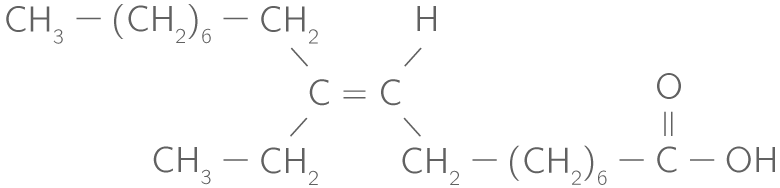
\includegraphics[width=0.5\textwidth]{figs/isomere_geometrique_synthese_chimie_sem1.png}
        \end{center}
        \item Les isomères \underline{optiques/énantiomères}. Ceux-ci sont
        l'image l'une de l'autre dans un mirroir et ne sont donc pas
        superposables. Une molécule a une énantiomère si elle possède un carbone
        asymétrique.
        \end{enumerate}

        Un carbone asymétrique est un carbone lié à 4 groupes différents. Si une
        molécule a $n$ carbones asymétriques, celle si a $2^n$ isomères.
        Attention, elle a $2^n$ isomères mais pas isomères optiques. Les
        isomères optiques ne viennent qu'en paires (chacune étant le reflet
        de l'autre dans un mirroir). --> $2^n$ isomères sous la forme de paire
        d'énantiomères.
       
        Une molécule est \underline{chirale} si elle comporte au moins un
        carbone asymétrique et, en conséquance, ne présente pas de plan de
        symétrie.

        Deux énantiomères dévient la lumière dans des directions différente.
        Un énantiomère est dit \underline{lévogyre} si elle la dévie vers la
        gauche et \underline{dextrogyre} quand elle la dévie vers la droite.

        Un mélange est dit \underline{racémique} quand il contient le même
        nombre d'énantiomères $L$ que $D$ d'un composé chirale.

    \subsection{Fonctions organiques} \label{ss:fct}

    Une \underline{fonction organique} est un atome ou un groupe d'atomes qui
    qui a des propriétés chimiques similaires à chaque fois qu'il est présent
    dans des composés différents. Il définit les caractéristiques physiques
    et chimique des molécules.
    
    Les fonctions vus au cours (le tiret signifie qu'il est relié à un (autre) 
    carbone de la chaine):


    Alcène \hspace{0.1\linewidth}\setchemfig{atom sep=1.7em}\chemfig{C=C} \newline

    Alcool \hspace{0.1\linewidth}\setchemfig{atom sep=1.7em}\chemfig{-OH} \newline

    Ether \hspace{0.1\linewidth}\setchemfig{atom sep=1.7em}\chemfig{R'-O-R} \newline

    Aldéhyde \hspace{0.1\linewidth}\setchemfig{atom sep=1.7em}\chemfig{-C=O} \newline

    Cétone \hspace{0.1\linewidth}\setchemfig{atom sep=1.7em}\chemfig{-C(=[2]O)-} \newline

    Acide Carboxylique \hspace{0.1\linewidth}\setchemfig{atom sep=1.7em}\chemfig{-C(=[1]O)(-[7]OH)} \newline

    Ester \hspace{0.1\linewidth}\setchemfig{atom sep=1.7em}\chemfig{-C(=[1]O)(-[7]O-R')} \newline

    Amines \hspace{0.1\linewidth}\setchemfig{atom sep=1.7em}\chemfig{-NH_2} \newline

    Amides \hspace{0.1\linewidth}\setchemfig{atom sep=1.7em}\chemfig{-C(=[1]O)(-[7]NH_2)} \newline

    Acide Amine \hspace{0.1\linewidth}\setchemfig{atom sep=1.7em}\chemfig{-C(-[6]NH_2)(-[1]C(=[1]O)(-[7]OH))} \hspace{2em}(Carbone avec acide carbo et amine)\newline

    Cycloalcane \hspace{0.1\linewidth}\setchemfig{atom sep=1.7em}\chemfig{C*5(-C-C-C-C-C)}, \hspace{2em} \setchemfig{atom sep=1.7em}\chemfig{C*6(-C-C-C-C-C-C)} \hspace{2em} etc.

    Aromatique \hspace{0.1\linewidth}\setchemfig{atom sep=1.7em}\chemfig{C*6(=C-C=C-C=C-C)} \newline
    \subsection{Halogènes}
    Les halogènes sont des atomes avec 7 de valence. Ceux-ci peuvent, comme
    l'hydrogène, remplir à eux seuls une liaison d'un carbone.

    Dans les halogènes, on peut compter le fluor \ce{F}, le chlore \ce{Cl}, le
    brome \ce{Br} et l'iode \ce{I}.

    \subsection{Nomenclature}

    Le nom du molécule comporte trois parties \newline

    \centerline{préfixe(s) -- radicale -- suffixe}

    \subsubsection{Préfixe}
    Le préfixe sera déterminer par les ramifications et les halogènes (les
    substituants) de la chaine. Chaque substituant différent correspondra à un
    chaînon dans le préfixe. 

    Ce chaînon sera, pour les ramification, le préfixe correspondant au nombre
    de carbones qu'ils comportent (meth, eth, but...) suivit de "yl" (pour 
    alkyle). 

    Pour les halogènes, il sera le nom de l'élément (brome, iode...) mais
    avec un "o" à la place de e final (bromo, fluoro...).

    Pour chaque chaînon différent, compter combien de substituants il
    représente et en fonction de cela, rajouter le préfixe \textit{di},
    \textit{tri}, \textit{tetra} ou
    aucun.

    Finalement, le préfixe sera la composition de tous les chainons par ordre
    alphabétique.

    \subsubsection{Radicale}
    Le radicale prend le nom (selon la nomenclature des alcanes) de la chaine
    carbonnée la plus longue comportant la fonction. S'il y a un cycle, il est
    automatiquement la chaine principale --le reste est considéré comme des
    alkyle/ramifications-- et il faut rajouter cyclo devant le nom qu'il a en
    tant qu'alcane.

    \subsubsection{Suffixe}
    Le suffixe est déterminer par la fonction.

    \begin{tabular}{ |p{4.5cm}|p{4.5cm}|}
        \hline
        \multicolumn{2}{|c|}{Tableau des fonctions} \\
        \hline
        Fonction & Suffixe\\
        \hline
        Alcène      & ène \\
        Alcyne      & yne \\
        Alcool      & ol \\
        Aldéhyde    & al \\
        Cétone      & one \\
        Amines       & amine \\
    \hline
    \end{tabular}

    Le suffixe des acides Carboxylique, des Esters et des Ether est plus
    complexe à trouver et sera directement vu dans la mise en commun.

    \subsubsection{Mise en commun}
    Pour mettre le préfixe, la racine et le suffixe en commun, il faut :

    Numéroter la chaine principale afin que le groupe fonctionnel ait le numéro
    le plus petit possible. Si ce n'est pas assez pour trouver le sens de
    numérotation, numéroter de sorte que le premier substituant ait le nombre
    le plus petit. Si ce n'est pas assez, refaire pour que le deuxième
    substituant ait le nombre le plus petit et ainsi de suite.

    Finalement, si il n'y a toujours pas moyen de trouver le sens de
    numérotation pour la molécule, numéroter pour que attribuer le plus petit
    indice au premier substituant en ordre alphabétique.

    Préciser pour chaque chaînon les/l'indice(s) du/des substituant(s) qu'il
    représente. Pour ce faire, on indique les numéros séparés par des virgules
    devant lui entre des tirets.

    Ensuite, on colle le radical au préfixe et on lui enlève son "e" final du
    "ane".

    Finalement, on ajoute le suffixe derrière le radical. Parfois, quand la
    position de la fonction est ambigue, on ajoute entre les deux son indice
    entouré de tirets.

    S'il y a plusieurs fonctions identiques, on utilise la même technique que
    pour les substituants, càd indiquer les différents indices et ajouter le
    préfixe \textit{di, tri} ou \textit{tetra}.

    Pour les acides carboxylique, on rajoute le suffixe "oïque" et on introduit
    le nom de la molécule par acide (ex acide butanoïque).

    Pour les Esters, le préfixe est "oate", et on rajoute après "d'/de [nom
    Alkyle R'] (ex méthanoate d'éthyle)

    Pour les Ethers, on utilise la nomenclature Alk + "oxy" + alcane, où "alk"
    est préfixe (meth, but...) de l'Alkyle (la chaine la moins longue des deux
    reliées à l'oxygène).  Alcane est le nom sous-forme alcane de la chaine
    principale/la plus longue. (ex methoxyéthane, ethoxyétane...) 

    \subsubsection{Quelques exemples}
    \vspace{2.5in}
    \subsection{Les grandes réactions}
    \subsubsection{Réaction d'addition}
    Une réaction d'addition est une réaction au cours de laquelle on lève une
    insaturationn et on la comble par deux hydrogènes/halogènes/alcool/autres.
    \subsubsection{Réaction d'élimination}
    Une réaction d'élimination est une foncièrement l'inverse de la réaction
    d'additino. On sature et forme un alcène/yne en libèrant deux éléments.
    Souvent les deux éléments vont former de l'eau ce qui est par exemple le cas
    quand on libère un hydrogène et une fonction alcool. 
    \subsubsection{Réaction de condensation avec élimination}
    Une réaction au cours de laquelle deux molécules fusionnent pour en former
    qu'une en relachant un sous-produit (généralement de l'eau).
    \subsubsection{Hydrolyse}
    Inverse de la réaction de condensation avec élmination. De l'eau se fait
    absorber et casse la molécule en deux.
    \subsubsection{Réaction d'oxydation}
    Une réaction d'oxydation est une réaction au cours de laquelle le niveau
    d'oxydation augmente.

    Le niveau d'oxydation correspond au nombres de liaisons qu'il y a avec
    l'oxygène. De cette manière, les saturations comptent double.

    \subsubsection{Réduction} 
    L'inverse d'une réaction d'oxydation ; le niveau d'oxydation diminue.
    \subsubsection{Substitution}
    On remplace un atome par un autre

    \ce{Alcool + NH_3 <-> Amine + H_2O}

    \subsection{Propriétés des molécules}
        Au plus une molécule est longue, au plus la température d'ébulition est élevée. Les molécules avec des coudes (alcènes) ont une température moins élevée. Les molécules polaires ont une température plus élevée à cause des interactions.

        Au plus un molécule est polaire, au plus elle se dissous dans l'eau. Un alcool plus long est moins polaire et se dissous moins bien. Au plus un alcane est long, au moins il est soluble aussi.

        Ainsi, les acides carboxyliques sont très solubles

    \begin{itemize}
        \item Au plus le nombre de carbones est grand, au plus la température d'ébulition est haute.
        \item Les alcènes ont une température d'ébulition plus basse grâce à leur coude.
        \item Les alcools sont polaires donc se mélangent mieux à l'eau (polaire aussi). Leur polarié rend leur température d'ébulition plus élevée.
        \item Au plus un alcane est long, au moins il est soluble
        \item Les acides Carboxylique ont encore plus d'oxygènes et sont ainsi encore plus polaires et sont plus solubles dans l'eau.
    \end{itemize}


\end{document}
